\twocolumn
\chapter{Mathematical Stuff}
\section{Trigonometric Values}
\begin{tikzpicture}
\coordinate (A) at (2cm, 0cm);
\coordinate (B) at (2cm, 4cm);              
\coordinate (C) at (0cm, 2cm);
\coordinate (D) at (4cm, 2cm);
\node at (2.5cm,2.5cm) {A};
\node at (1.5cm,2.5cm) {S};
\node at (1.5cm,1.5cm) {T};
\node at (2.5cm,1.5cm) {C};
\draw (A) -- (B);
\draw (C) -- (D);
\draw (2cm, 2cm) circle (1.2cm);
\end{tikzpicture}
    
\def\arraystretch{1.5}
\begin{tabular}{ |c|c|c|c|c| } 
\hline
\textbf{rad}	& \textbf{$\degrees$}	& \textbf{sin} 		& \textbf{cos} 	& \textbf{tan} 	\\ 
\hline
$ 0 $	 		& 0		& $0$ 			& $1$	 			& $0$ 							\\
\hline
$\pi/6 $ 		& 30	& $1/2$ 		& $\sqrt{3}/2 $ 	& $1/\sqrt{3}$ 					\\
\hline
$\pi/4 $ 		& 45	& $1/\sqrt{2}$ 	& $1/\sqrt{2} $ 	& $1$							\\
\hline
$\pi/3 $ 		& 60	& $\sqrt{3}/2$ 	& $ 1/2 $	 		& $\sqrt{3}$					\\
\hline
$\pi/2 $ 		& 90	& $1$ 			& $ 0 $ 			& $\pm\infty$					\\
\hline
$2\pi/3 $ 		& 120	& $\sqrt{3}/2$	& $ -1/2 $ 			& $-\sqrt{3}$					\\
\hline
$3\pi/4 $ 		& 135	& $1/\sqrt{2}$	& $ -1/\sqrt{2} $ 	& $-1$							\\
\hline
$5\pi/6 $ 		& 150	& $1/2$			& $ -\sqrt{3}/2 $ 	& $-1/\sqrt{3}$					\\
\hline
$\pi $ 			& 180	& $0$			& $ -1 $		 	& $0$							\\
\hline
$7\pi/6 $ 		& 210	& $-1/2$		& $ \sqrt{3}/2 $	& $1/\sqrt{3}$					\\
\hline
$5\pi/4 $ 		& 225	& $-1/\sqrt{2}$	& $ -1/\sqrt{2} $	& $1$							\\
\hline
$4\pi/3 $ 		& 240	& $-\sqrt{3}/2$	& $ -1/2 $			& $\sqrt{3}$					\\
\hline
$3\pi/2 $ 		& 270	& $-1$			& $ 0 $				& $\pm\infty$					\\
\hline
$5\pi/3 $ 		& 300	& $-\sqrt{3}/2$	& $ 1/2 $			& $-\sqrt{3}$					\\
\hline
$7\pi/4 $ 		& 315	& $-1/\sqrt{2}$	& $	1/\sqrt{2} $	& $-1$							\\
\hline
$11\pi/6 $ 		& 330	& $-1/2$		& $ \sqrt{3}/2 $	& $-1/\sqrt{3}$					\\
\hline
$2\pi $ 		& 360	& $0$			& $ 1 $		 		& $0$							\\
\hline
\end{tabular}      
                   
\subsection{Pythagorean Triples}

\begin{tikzpicture}[scale=1.25]%,cap=round,>=latex]
\coordinate (A) at (0cm,-3.46cm);
\node at (0.2cm,-3.15cm) {$\frac{\pi}{2}$};
\coordinate (B) at (0cm, 0cm);
\node at (0.2cm, -0.8cm) {$\frac{\pi}{6}$};
\coordinate (C) at (2cm,-3.46cm);
\node at (1.5cm, -3.15cm) {$\frac{\pi}{3}$};
\draw (A) -- node[left] {$\sqrt{3}$} (B) -- node[right] {$2$} (C) -- node[below] {$1$} (A);
                
\coordinate (D) at (3cm,-3.46cm);
\node at (3.2cm,-3.15cm) {$\frac{\pi}{4}$};
\coordinate (E) at (3cm, -1.46cm);
\node at (3.2cm, -2cm) {$\frac{\pi}{4}$};
\coordinate (F) at (5cm,-3.46cm);
\node at (4.3cm, -3.15cm) {$\frac{\pi}{2}$};
\draw (D) -- node[left] {$1$} (E) -- node[above] {$\sqrt{2}$} (F) -- node[below] {$1$} (D);
                
\end{tikzpicture}

\onecolumn

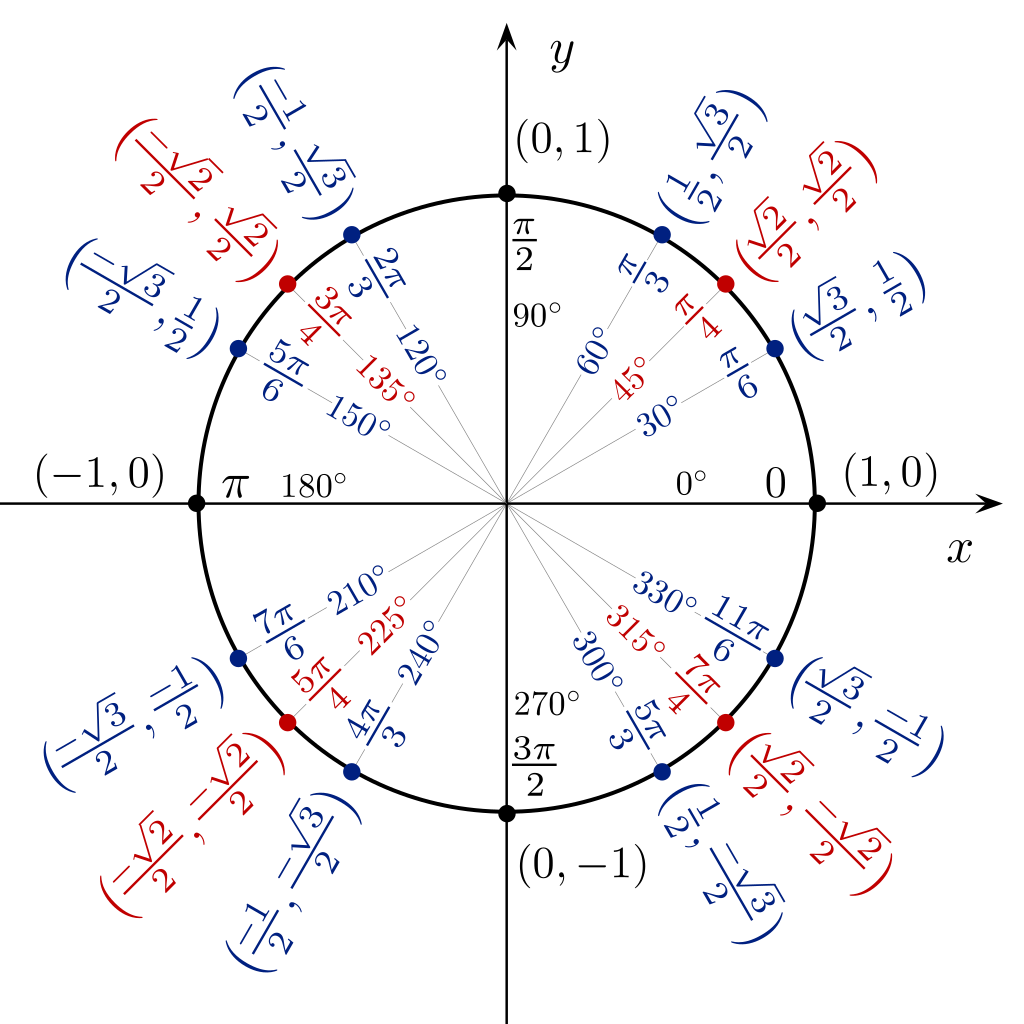
\includegraphics[width=\textwidth]{figures/1024px-Unit_circle_angles_color_svg.png}